\chapter{Over Sensor Maritime}
Sensor Maritime is een bedrijf dat zicht focust op research en development in de maritieme sector. Sensor Maritime is een van de vier bedrijven die deel uitmaken van de Sensor Groep, deze groep bestaat uit Sensor Maritime, Sensor BV, Sensor Partners, en Vision Partners. Wat deze bedrijven met elkaar gemeen hebben, is dat deze allemaal gefocust zijn op het ontwikkelen van nieuwe technologieën met verschillende sensoren. Sensor Maritime heeft een kantoor en is op het moment gebaseerd in Vught. Het bedrijf bestaat uit 4 mensen en heeft drie afdelingen:
\begin{enumerate}
	\item Sales
	\item Service
	\item Research en Development
\end{enumerate}
Tijdens de afstudeerstage zal de afstudeerder alleen betrokken zijn bij Research and Development.
\newline

\noindent Sensor Maritime is niet anders dan een sensor georiënteerd bedrijf, deze zijn specifiek gefocust op het ontwikkelen van sensorsystemen voor binnenvaartschepen. De klant van Sensor Maritime zijn dan ook kapiteinen van binnenvaartschepen \ref{fig:customer_sensor_maritime}.
\begin{figure}[h!]

	\centering
	\caption{Klant van Sensor Maritime}
	\label{fig:customer_sensor_maritime}
	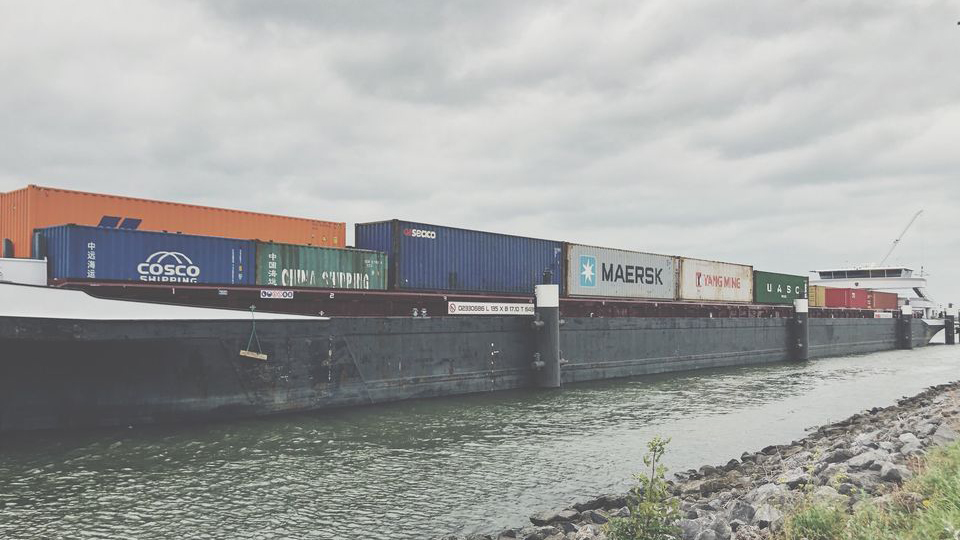
\includegraphics[width=0.7\linewidth]{about/binnevaart.jpg}
	

\end{figure}

\noindent Projecten waar Sensor Maritime momenteel bezig mee zijn is bijvoorbeeld, een systeem om objecten aan de zijkanten van een schip te kunnen detecteren en deze te tekenen op een scherm. Daarnaast is Sensor Maritime ook bezig met een systeem om objecten aan de voorkant van een schip te kunnen detecteren, en een systeem om te kunnen detecteren of een schip onder een brug door kan met de stuurhut.
